% !TEX root = ./Vorlesungsmitschrift DIFF 2.tex  
\chapter{Differentialgleichungen}
\lecture{Do 11.06. 10:15}{}
\begin{definition}\label{dgl}\index{Differentialgleichung 1. Ordnung}
  \( V\subset \reals^{n+1} \), \( F\maps V\to \reals^n \) stetig. Dann nennt man
  \begin{equation*}
    x'=F(t,x)\tag{\(*\)}\label{eq:erste_diffgleichung}
  \end{equation*}
  eine \emph{Differentialgleichung (DGL) \ordinalnum{1} Ordnung} (\( n=1 \)) oder \emph{System von DGL'n \ordinalnum{1} Ordnung} (\( n\geq 2 \)). Eine \emph{Lösung} von \eqref{eq:erste_diffgleichung} ist eine differenzierbare Funktion \( u\maps I\to \reals^n \), \( I\subset \reals \) Intervall, mit \( u'(t)=F(t,u(t)) \), also insbesondere \( (t,u(t)) \in V\), also
  \begin{equation*}
    \Gamma_u=\Set{(t,u(t))|t\in I}\subset V.
  \end{equation*}
\end{definition}
\section{Geometrische Interpretation}
Sei zunächst \( F \) nicht von \( t \) abhängig, \( F\maps \reals*U\to \reals^n \), \( U\subset \reals^n \) offen, \( T(t,x)=G(x) \), also
\begin{equation*}
  x'=G(x)\tag{\(**\)}\label{eq:zeitunabhaengige_diffgleichung}.
\end{equation*}
Dann kann man \( G \) als Vektorfeld auf \( U \) ansehen (denn \( \tangentialraum-{U}=\Span-{\set{e_1,\dotsc,d_n}} \)), in diesem Fall ein \emph{stetiges Vektorfeld}, also eine stetige Abbildung \( G\maps  U \to \tangentialraum-{U}=\reals^n \). Eine Lösung der DGL \eqref{eq:zeitunabhaengige_diffgleichung} ist dann eine differenzierbare Integralkurve (nicht unbedingt stetig differenzierbar).
\begin{figure}[H]
  \centering
  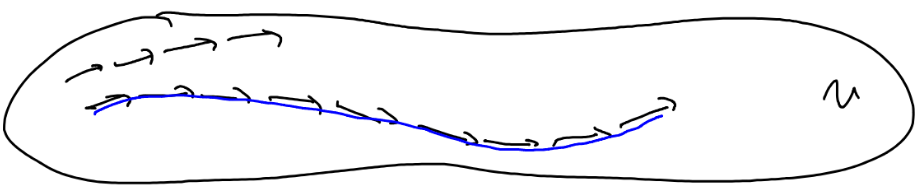
\includegraphics[width=0.7\linewidth]{dgl_loesung_als_integralkurve}
  \label{fig:dgl_loesung_als_integralkurve}
\end{figure}
\begin{beispiel*}
  \( G\maps \reals^2\to \reals^2 \), \( G(x_1,x_2)=\begin{pNiceMatrix} -x_2 \\ x_1 \end{pNiceMatrix} \).
  \begin{figure}[H]
    \centering
    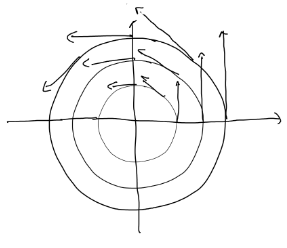
\includegraphics[width=0.5\linewidth]{kreis_dgl}
    \label{fig:kreis_dgl}
  \end{figure}
  Hier raten wir:
  \begin{equation*}
    u(t)=\begin{pNiceMatrix} \Cos{t} \\ \Sin{t} \end{pNiceMatrix}\cdot r\quad r>0.
  \end{equation*}
  Tatsächlich
  \begin{align*}
    u'(t)&=\begin{pNiceMatrix} -\Sin{t} \\ \Cos{t} \end{pNiceMatrix}\cdot r\quad r>0\\
    &=G(u(r)).
  \end{align*}
  Man kann sich vorstellen, während Zeit \( t \) vergeht, wandert ein Punkt entlang von \( u \) und erfüllt zu jedem Zeitpunkt \( t \), dass seine Geschwindigkeit in Richtung und Größe durch \( G \) vorgegeben ist (und wie wir sehen werden unter gewissen Umständen \( u \) selbst dadurch eindeutig festgelegt wird). 
  
  Dieses Bild trägt auch noch, wenn \( F \) explizit von \( t \) abhängt:\\
  In diesem Fall verändert sich das Vektorfeld selbst, während Zeit verstreicht, und der Tangentialvektor, dem \( u'(t) \) zum Zeitpunkt \( t \) gleich sein soll, ist nicht nur von der Position \( \gamma(t) \) abhängig, sondern auch om Zeitpunkt \( t \).
\end{beispiel*}
\begin{beispiele*}
  \begin{enumerate}
    \item Aus dem Satz über implizite Funktionen berechnete Ableitung der Auflösungsfunktion \( g \), etwa in Vorlesung 9 (\hyperref[implizite_funktion_beispiel_fuer_dgls]{\ordinalnum{1} Beispiel vor \thref{satz_von_der_umkehrabbildung}})
    \begin{equation*}
      y'=\begin{pNiceMatrix} \frac{t}{y} &  \\  & \frac{t}{y} \end{pNiceMatrix}.
    \end{equation*}
    \item Wachstumsmodelle:
    \begin{eigenschaftenenumerate}
      \item Wachstum proportional zur Populationszahl
      \begin{equation*}
        x'=\alpha x,\quad u(t)=c e^{\alpha t}.
      \end{equation*}
      \item Logistisches Wachstum (Grenzen des Wachstums wegen Ressourcen-Knappheit). Wachstum ist proportional zur Populationszahl \( y \) und zum verbleibenden Platz \( \mu(1-y) \).
      \begin{equation*}
        x'=\alpha x(1-x).
      \end{equation*}
      \item Räuber-Beute-Modelle
    \end{eigenschaftenenumerate}
    \item Jede Menge Modelle in Physik, Chemie, Biologie, Wirtschaft \etc, \zb freier Fall (\ordinalnum{2} Ableitung)
    \begin{equation*}
      x''=-g.
    \end{equation*}
  \end{enumerate}
  Die DGL'n, die wir hier betrachte, werden explizit lösbar sein, \dh es gibt Lösungen \( u \), die man explizit angeben kann. Für Räuber-Beute-Modell etwa gibt es solche aber \ia nicht.
\end{beispiele*}
\section{Existenz- und Eindeutigkeitssatz}
Sei \( x'=F(t,x) \) eine DGL wie in \thref{dgl},
\begin{equation*}
  F\maps V\to \reals^n, V\subset \reals\times \reals^n.
\end{equation*}
Legt man zusätzlich fest, dass eine Lösung
\begin{equation*}
  u\maps I\to \reals^n
\end{equation*}
erfüllen soll, dass \( u(t_0)=u_0 \) gelten soll für ein \( (t_0,u_0)\in V \), so spricht man on einem \emph{Anfangswertproblem} (AWP) und notiert
\begin{equation*}
  \begin{gathered}
    x'=F(t,x)\\
    x(t_0)=u_0
  \end{gathered}\tag{\(*\)}\label{eq:awp}
\end{equation*}
\begin{beispiel*}
  \( x'=\alpha x \), \( u(t)=c e^{\alpha t} \) löst die DGL\@. \( u(t)=u_0 e^{\alpha t} \) löst das AWP \( x'=\alpha x \), \( x(0)=u_0 \).
\end{beispiel*}
Existenz und Eindeutigkeit der Lösung: \\
Formuliere das Problem als Fixpunkt-Problem und verwende den Banachschen Fixpunktsatz.

Denn \( u \) ist eine Lösung der DGL \( x'=F(t,x) \)
\begin{equation*}
  \iff u(t)=u(t_0)+\Integrate{u'(s)}{s,t_0,t}=u(t_0)+\Integrate{F(s,u(s))}{s,t_0,t}
\end{equation*}
und löst \( u \) das AWP \eqref{eq:awp}, so ist \( u(t_0)=u_0 \). \( u \) ist also Lösung des AWP \tiff \( u= \) Fixpunkt der Abbildung
\begin{equation*}
  u\mapsto Tu,\quad Tu(t)=u_0+\Integrate{F(s,u(s))}{s,t_0,t}.
\end{equation*}
\begin{definition}\index{lipschitz-Bedingung}
  Sei \( V\subset \reals\times \reals^n \) und \( F\maps V\to \reals^n  \) eine Funktion. Man sagt
  \begin{itemize}
    \item \( F \) erfüllt auf \( V \) eine \emph{Lipschitz-Bedingung} mit Lipschitz-Konstante \( L \), falls es \( L\geq 0 \) gibt \sd 
    \begin{equation*}
      \norm{F(t,x)-F(t,\tilde{x})}\leq L\norm{x-\tilde{x}}\quad \forall (t,x),(t,\tilde{x})\in V.
    \end{equation*}
    \item \( F \) erfüllt \emph{lokal eine Lipschitz-Bedingung}, falls es zu jedem Punkt \( (t_0,x_0)\in V \) eine offene Umgebung \( \tilde{V} \) und eine Konstante \( L=L_{\tilde{V}}\geq 0 \) gibt \sd \( F \) auf \( V\cap \tilde{V} \) eine Lipschitz-Bedingung mit Konstante \( L \) erfüllt. 
  \end{itemize}
\end{definition}
\begin{lemma}
  Ist \( V\subset \reals\times \reals^n \) offen und ist \( F\maps V\to \reals^n \) bezüglich der hinteren \( n \) Variablen stetig differenzierbar, so erfüllt \( f \) lokal in \( V \) eine Lipschitz-Bedingung.
\end{lemma}
\begin{proof}
  Sei \( (t_0,x_0) \in V\). Dann \texists \( r>0 \) \sd
  \begin{equation*}
    K\definedas \Set{(t,x)\in V|\abs{t-t_0}\leq r \text{ und }\norm{x-x_0}\leq r}.
  \end{equation*}
  \( K \) ist kompakt nach dem Satz von Heine + Borel.
  \begin{equation}
  \implies L\definedas \sup_{(t,x)\in K}\norm{D_2 F}<\infty\quad DF=\begin{pNiceMatrix} \partial_1 f & D_2 F \end{pNiceMatrix}.
  \end{equation}
  MWS \timplies \( \norm{F(t,x)-F(t,\tilde{x})}\leq L\norm{x-\tilde{x}} \).
  
\end{proof}
\begin{bemerkung*}
  Stetige Differenzierbarkeit bezüglich der hinteren \( n \) Variablen bedeutet, dass \( D_2 F \) auch bezüglich der ersten Variablen stetig ist.
\end{bemerkung*}
\begin{satz}[Picard-Lindelöf]\label{picard-lindeloef}\index{Satz von Picard-lindelöf}
  Sei \( V\subset \reals\times \reals^n  \). Sei \( mF\maps V\to \reals^n \) stetig und erfülle lokal auf \( V \) eine Lipschitz-Bedingung. Dann hat das Anfangswertproblem
  \begin{align*}
    x'&=F(t,x)\\
    x(t_0)&=u_0\quad (t_0,u_0)\in V.
  \end{align*}
  ine eindeutige Lösung \( u\maps I\to \reals^n \) mit \( t_0\in I \) und \( u(t_0)=u_0 \).
\end{satz}
\begin{proof}
  Da \( F \) lokal einer Lipschitz-Bedingung genügt, gibt es \( L\geq 0 \) und eine Umgebung \( \tilde{V} \) von \( (t_0,x_0) \) \sd
  \begin{equation*}
    \norm{F(t,x)-F(t,\tilde{x})}< L\norm{x-\tilde{x}}\quad \forall (t,x),(t,\tilde{x})\in \tilde{V}\cap V.
  \end{equation*}
  Sei \( J\times K\subset \tilde{V}\cap V \) mit \( J \) kompaktes Intervall \( t_0\in J \), \( K\subset \reals^n \) kompakt, \( x_0\in K \), \obda \( K=\abschluss{B_r(x_0)} \), \( r>0 \). 
  
  Wähle \( \delta>0 \) \sd
  \begin{equation*}
    L\delta<1 \text{ und }\delta\norm{F}_{\infty, J\times K}\leq r.
  \end{equation*}
  Betrachte \( T\maps \mathcal{F}\to \stetigefunktionen(I,\reals^n) \),
  \begin{equation*}
    \mathcal{F}=\Set{u\in \stetigefunktionen(I,\reals^n)|u(I)\subset K}
  \end{equation*}
  mit \( I=J\cap \interval{t_0-\delta}{t_0+\delta} \) (kompakt).
  \begin{equation*}
    (Tu)(t)=u_0+\Integrate{F(s,u(s))}{s,t_0,t}.
  \end{equation*}
  Es ist tatsächlich \( Tu\in \stetigefunktionen(I,\reals^n) \). Sei \( u\in I \) und \( t\in I \). Dann gilt
  \begin{align*}
    \supnorm{Tu-u_0}&=\supnorm*{\Integrate{F(s,u(s))}{s,t_0,t}}\\
    &\leq \delta\supnorm{F}\leq r,
  \end{align*}
  somit ist \( Tu\in \mathcal{F}\quad \forall u\in \mathcal{F} \). Zudem ist 
  \begin{align*}
    \supnorm{Tu-Tv}&=\supnorm*{\Integrate{(F(s,u(s))-F(s,v(s)))}{s,t_0,t}}\\
    &\leq\abs{t-t_0}L\supnorm{u-v}\\
    &\leq \braceannotate{\leq L\cdot \delta<1}{L\cdot \abs{I}\cdot\supnorm{u-v}}.
  \end{align*}
  \timplies \( T\maps \mathcal{F}\to \mathcal{F} \) ist Kontraktion. Zudem ist \( \mathcal{F}\subset \stetigefunktionen(I,\reals^n) \)   abgeschlossen (bezüglich \( \supnorm{\cdot} \)) \timplies \Beh (Banachscher Fixpunktsatz).

  
\end{proof}
\begin{bemerkung*}
  Der Beweis ist konstruktiv, \dh beginnend mit \( u_0(t)=u_0 \) (\zb) erhält man die Lösung als gleichmäßigen Limes der Iteration
  \begin{equation*}
    u_{n+1}(t)=u_0+\Integrate{F(s,u_n(s))}{s,t_0,t.}
  \end{equation*}
\end{bemerkung*}
\begin{beispiele*}
   \begin{enumerate}
     \item \( x'=\begin{pNiceMatrix} -x_2 \\ x_ 1\end{pNiceMatrix} \), \( x(0)=\begin{pNiceMatrix} 1 \\ 0 \end{pNiceMatrix} \).
     \begin{align*}
       u_0(t)&=\begin{pNiceMatrix} 1 \\ 0 \end{pNiceMatrix}\\
       u_1(t)&=\begin{pNiceMatrix} 1 \\ 0 \end{pNiceMatrix}+\begin{pNiceMatrix} -\Integrate{0}{s,0,t} \\ \Integrate{1}{s,0,t} \end{pNiceMatrix}=\begin{pNiceMatrix} 1 \\ t \end{pNiceMatrix}\\
       u_2(t)&=\begin{pNiceMatrix} 1 \\ 0 \end{pNiceMatrix}+\begin{pNiceMatrix} -\Integrate{s}{s,0,t} \\ \Integrate{1}{s,0,t} \end{pNiceMatrix}=\begin{pNiceMatrix} 1-\frac{t^2}{2} \\ t \end{pNiceMatrix}.
     \end{align*}
     \begin{behauptung*}
       \begin{align*}
         u_{2u}(t)&=\begin{pNiceMatrix} 1-\frac{t^2}{2}+\dotsb+(-1)^n \frac{t^{2n}}{\factorial+{2n}} \\ t-\dotsb-(-1)^n\frac{t^{2n-1}}{\factorial+{2n-1}} \end{pNiceMatrix}\\
         u_{2n+1}(t)=\begin{pNiceMatrix} 1-\frac{t^2}{2}+\dotsb+(-1)^n\frac{t^{2n}}{\factorial+{2n}} \\ t-\dotsb+(-1)n\frac{t^{2n+1}}{\factorial+{2n+1}} \end{pNiceMatrix}.
       \end{align*}
     \end{behauptung*}
     \begin{proof}
      per Induktion       
     \end{proof}
     \begin{equation*}
       \implies x(t)=\begin{pNiceMatrix} \Cos{t} \\ \Sin{t} \end{pNiceMatrix}
     \end{equation*}
     \item \( F(t,x)=2tx \), \( F\maps \reals^2\to \reals \), \( x'=2tx \), \( x(0)=x_0 \).
     \begin{gather*}
       u_{k+1}(t)=x_0+2\Integrate{su_k(s)}{s,0,t}\\
       u_0(t)=x_0\implies \begin{aligned}[t]
         u_1(t)&=x_0+x_0t^2\\
         u_2(t)&=x_0+2\Integrate{s(x_0+x_0s^2)}{s,0,t}\\
         &=x_0\p*{ 1+t^2+\frac{t^4}{2} }.
       \end{aligned}
     \end{gather*}
     Per Induktion beweist man
     \begin{align*}
       &u_k(t)=x_0\p*{ 1+t^2+\frac{t^4}{2}+\frac{t^6}{\factorial{3}}+\dotsb+\frac{t^{2k}}{\factorial{k}} }\\
       \implies &u(t)=x_0 e^{t^2}.
     \end{align*}
   \end{enumerate}
\end{beispiele*}
\begin{definition*}\index{Differentialgleichung $k$-ter Ordnung}
  Sei \( V\subset \reals\times \reals^{k\cdot n} \), \( F\maps V\to \reals^n \) stetig. Dann nennt man
  \begin{equation*}
    x^{(k)}=F(t,x,x',x'',\dotsc,x^{(k-1)})\tag{\( * \)} \label{eq:dglkter}
  \end{equation*}
  eine \emph{Differentialgleichung (DGL) \( k \)-ter Ordnung} (\( n=1 \)) oder \emph{System von DGL'n \( k \)-ter Ordnung} (\( n\geq 2 \)).
  \begin{beispiel*}
    \( x''=-(x')^2+xt \) (\( k=2 \)) (also \( F(t,x_0,x_1)=-x_1^2+x_0t \)).
  \end{beispiel*}
  Eine Lösung von \eqref{eq:dglkter} ist eine \( n \)-mal differenzierbare Funktion \( \varphi\maps I\to \reals^n \) mit
  \begin{equation*}
    \varphi^{(k)}(t)=F(t,\varphi(t),\varphi'(t),\varphi''(t),\dotsc,\varphi^{(k-1)}(t)).
  \end{equation*}
  Damit dies wohldefiniert ist, muss gelten
  \begin{equation*}
    (t,\varphi(t),\varphi'(t),\varphi''(t),\dotsc,\varphi^{(k-1)}(t))\in V\quad \forall t\in I.
  \end{equation*}
\end{definition*}

\begin{bemerkung*}
  Wir können in Beweisen \obda \( k=1 \) setzen und alle Sätze, die wir für diesen Fall beweisen, auf den Fall \( k\geq 2 \) übertragen. Es gilt nämlich:
\end{bemerkung*}
\begin{satz}[Reduktion der Ordnung]\label{reduktion_der_ordnung}\index{Reduktion der Ordnung}
  Sei
  \begin{equation*}
    x^{(k)}=F(t,x,,x',\dotsc,x^{(k-1)})\tag{\(*\)}\label{eq:dglsyskter}
  \end{equation*}
  DGL (-System) \( k \)-ter Ordnung. Betrachte
  \begin{gather*}
    F\maps V\to \reals^{n\cdot k}\\
    \tilde{F}(t,x_0,x_1,\dotsc,x_{k-1})=\begin{pNiceMatrix} x_1 \\ x_2 \\ \Vdots \\ x_{k-1} \\ F(t,x_0,x_1,\dotsc,x_{k-1}) \end{pNiceMatrix}
  \end{gather*}
  und das DGL-System \ordinalnum{1} Ordnung
  \begin{equation*}
    \begin{pNiceMatrix} x_0 \\ x_1 \\ \Vdots x_{k-1} \end{pNiceMatrix}'=\tilde{F}(t,x_0,\dotsc,x_{k-1})=\begin{pNiceMatrix} x_1 \\ x_2 \\ \Vdots \\ x_{k-1} \\ F(t,x_0,x_1,\dotsc,x_{k-1}) \end{pNiceMatrix}\tag{\( ** \)}\label{eq:reduziertes_dglsys}
  \end{equation*}
  Sei \( u\maps I\to \reals^n \) eine Lösung von \( \eqref{eq:dglsyskter} \), gelte also
  \begin{equation*}
    u^{(k)}(t)=F(t,u(t),u'(t),u''(t),\dotsc,u^{(k-1)}(t)) \forall t\in I,
  \end{equation*}
  so ist
  \begin{equation*}
    \underline{U}\definedas \begin{pNiceMatrix} u \\ u' \\ \Vdots \\ u^{(k-1)} \end{pNiceMatrix}\maps I\to \reals^{k\cdot n}
  \end{equation*}
  eine Lösung von \eqref{eq:reduziertes_dglsys}. Umgekehrt: Sei
  \begin{equation*}
    \underline{U}\definedas \begin{pNiceMatrix} u_0 \\ u_1\\ \Vdots \\ u_{k-1} \end{pNiceMatrix}\maps I\to \reals^{k\cdot n}
  \end{equation*}
  Lösung von \eqref{eq:reduziertes_dglsys}, so ist \( u\definedas u_0\maps I\to \reals^n \) eine Lösung von \eqref{eq:dglsyskter}.
\end{satz}
\begin{beispiel*}
  \begin{equation*}
    x''+x=0\tag{\( * \)}\label{eq:zweierdgl_beispiel}
  \end{equation*}
  Lösungen: \( \Cos; \), \( \Sin; \). \( F(t,x,x')=-x \). Reduktion der Ordnung:
  \begin{gather*}
    \begin{pNiceMatrix} x_0 \\ x_1 \end{pNiceMatrix}'=\begin{pNiceMatrix} x_1 \\ F(t,x_0,x_1) \end{pNiceMatrix}=\begin{pNiceMatrix} x_1 \\ -x_0 \end{pNiceMatrix}\tag{\( ** \)}\label{eq:reduziertes_zweierdgl_beispiel}\\
    \begin{pNiceMatrix} \Sin; \\ \Cos; \end{pNiceMatrix}'(t)=\begin{pNiceMatrix} \Cos{t} \\ -\Sin{t} \end{pNiceMatrix},\quad \begin{pNiceMatrix} \Cos; \\ -\Sin; \end{pNiceMatrix}'(t)=\begin{pNiceMatrix} -\Sin{t} \\ -\Cos{t} \end{pNiceMatrix}
  \end{gather*}
  \timplies \( \Sin; \) und \( \Cos; \) sind Lösungen von \eqref{eq:reduziertes_zweierdgl_beispiel}.
\end{beispiel*}
\begin{bemerkung*}
  Wie man an der Formulierung des Satzes und des Beispiels sieht, ist es zum \emph{Lösen} einer DGL \( k \)-ter Ordnung in der Regel nicht opportun, die Ordnung zu reduzieren.
\end{bemerkung*}
\begin{proof}[Beweis von \thref{reduktion_der_ordnung}]
  Sei \( u\maps I\to \reals \) Lösung on \eqref{eq:dglsyskter}, \dh
  \begin{equation*}
    u^{(k)}(t)=F(t,u(t),u'(t),u''(t),\dotsc,u^{(k-1)}(t)).
  \end{equation*}
  Dann ist
  \begin{equation*}
    \underline{U}\maps I\to \reals^{k\cdot n},\quad \underline{U}(t)\definedas \begin{pNiceMatrix} u(t) \\ u'(t) \\ \Vdots \\ u^{(k-1)}(t) \end{pNiceMatrix}
  \end{equation*}
  eine Lösung von \eqref{eq:reduziertes_dglsys}, denn
  \begin{equation*}
    \underline{U}'(t)=\begin{pNiceMatrix} u'(t) \\ u''(t)\\ \Vdots \\ u^{(k)}(t) \end{pNiceMatrix}=\begin{pNiceMatrix} u'(t) \\ \Vdots \\ u^{(k-1)}(t)\\ F(t,u(t),u'(t),u''(t),\dotsc,u^{(k-1)}(t)) \end{pNiceMatrix}.
  \end{equation*}
  Sei umgekehrt \( \underline{U}\maps I\to \reals^k \), \( \underline{U}(t)=\begin{pNiceMatrix} u_0(t) \\ \vdots \\ u_{k-1}(t) \end{pNiceMatrix} \) eine Lösung on \eqref{eq:reduziertes_dglsys}, gelte also
  \begin{equation*}
    \underline{U}'(t)=\begin{pNiceMatrix} u_0'(t) \\ \Vdots \\ u_{k-1}'(t) \end{pNiceMatrix}=\begin{pNiceMatrix} u_1(t) \\ \Vdots \\ u_{k-1}(t)\\ F(t,u(t),u'(t),u''(t),\dotsc,u^{(k-1)}(t)) \end{pNiceMatrix},
  \end{equation*}
  dann ist \( u\definedas u_0 \) eine Lösung von \eqref{eq:dglsyskter}, denn
  \begin{align*}
    u_0'(t)&=u_1(t)\\
    u_1'(t)&=u_2(t)\text{ und } u_1'(t)=u_0''(t)\\
    &\vdots
    u_{k-2}'(t)&=u_{k-1}(t)\text{ und }u_{k-2}'(t)=u_{k-3}''(t)=\dotsb=u_0^{(k-1)}(t)\\
    u_{k-1}(t)=F(t,u(t),\dotsc,u^{(k-1)}(t))\text{ und }u_{k-1}'=u_0^{(k)}(t).
  \end{align*}
\end{proof}
\begin{bemerkung*}[Ergänzend (wie in der \enquote{Vorlesung} vom 11.06.\ und weitere Bemerkungen (\tto nächstes Mal))]
  Man sieht aus dem Beweis, dass
  \begin{equation*}
    \underline{U}(t)\definedas \begin{pNiceMatrix} u(t) \\ u'(t) \\ \Vdots \\ u^{(k-1)}(t) \end{pNiceMatrix}
  \end{equation*}
  mit \( u \) Lösung von \eqref{eq:dglsyskter} genau dann Lösung mit Anfangswert \( \underline{U}(t_0)=\begin{pNiceMatrix} v_0 \\ v_1 \\ \Vdots \\ v_{k-1} \end{pNiceMatrix} \) ist, wenn
  \begin{align*}
    u(t_0)&=v_0\\
    u'(t_0)&=v_1\\
    &\vdots\\
    u^{(k-1)}(t_0)&=v_{k-1},
  \end{align*}
  also wenn bei der Lösung von \eqref{eq:dglsyskter} alle Ableitungen bis zur \( (k-1) \)-sten fest liegen.
\end{bemerkung*}
\begin{bemerkung*}
  Erfüllt \( F \) lokal eine Lipschitz-Bedingung, so auch \( \tilde{F} \), denn
  \begin{align*}
    \euclidiannorm{\tilde{F}(t,x_0,\dotsc)-\tilde{F(t,\tilde{x_0},\dotsc)}}&\definedas C\sum_{j=0}^{k-1}\euclidiannorm{x_j-\tilde{x}_j}+C\euclidiannorm{\tilde{F}(\dotsc)-\tilde{F}(\dotsc)}\\
    &\leq C\euclidiannorm{\tilde{F}(\dotsc)-\tilde{F}(\dotsc)}.
  \end{align*}
  Es folgt: Erfüllt \( F \) lokal eine Lipschitz-Bedingung, so hat das AWP
  \begin{gather*}
    x^{(k)}=F(t,x,x',\dotsc, x^{(k-1)})\\
    x(t_0)=v_0,x'(t_0)=v_1,\dotsc,x^{(k-1)}=v_k
  \end{gather*}
  mit \( (t_0,v_0,v_1,\dotsc,_k)\in V\subset \reals^{nk+1} \) eine eindeutige Lösung.
\end{bemerkung*}  